\documentclass[a5paper]{article}
\usepackage[a5paper, top=8mm, bottom=8mm, left=8mm, right=8mm]{geometry}

\usepackage{polyglossia}
\setdefaultlanguage[babelshorthands=true]{russian}

\usepackage{fontspec}
\setmainfont{FreeSerif}
\newfontfamily{\russianfonttt}[Scale=0.7]{DejaVuSansMono}

\usepackage[font=scriptsize]{caption}

\usepackage{amsmath}
\usepackage{amssymb,amsfonts,textcomp}
\usepackage{xcolor}
\usepackage{array}
\usepackage{hhline}
\usepackage{cite}

\usepackage[hang,multiple]{footmisc}
\renewcommand{\footnotelayout}{\raggedright}

\PassOptionsToPackage{hyphens}{url}\usepackage[xetex,linktocpage=true,plainpages=false,pdfpagelabels=false]{hyperref}
\hypersetup{colorlinks=true, linkcolor=blue, citecolor=blue, filecolor=blue, urlcolor=blue, pdftitle=1, pdfauthor=, pdfsubject=, pdfkeywords=}

\usepackage{tabu}

\tabulinesep=1.2mm

\usepackage{graphicx}
\usepackage{indentfirst}
\usepackage{multirow}
\usepackage{subfig}
\usepackage{footnote}
\usepackage{minted}

\newcommand{\attribution}[1] {
\vspace{-5mm}\begin{flushright}\begin{scriptsize}\textcolor{gray}{\textcopyright\, #1}\end{scriptsize}\end{flushright}
}

\sloppy
\pagestyle{plain}

\title{Экосистема open source проектов}
\author{Юрий Литвинов\\\small{yurii.litvinov@gmail.com}}

\date{06.02.2019}

\begin{document}

\maketitle
\thispagestyle{empty}

\section{Введение}

В этой лекции пойдёт речь об инструментах, которые призваны облегчить open source (и не только) разработку --- системы непрерывной интеграции, облачные анализаторы кода, всякие инфраструктурные штуки типа средств планирования и средств общения разработчиков. Все рассматриваемые сегодня инструменты бесплатны для open source и широко используются, поэтому рекомендуются и к использованию в домашках (некоторые даже настоятельно рекомендуются, CI будет обязательна). Обзор, естественно, далеко не полон, таких штук существенно больше, чем будет сегодня рассказано, и даже не факт, что будет рассказано про лучшие --- выбор инструментов, о которых пойдёт речь сегодня, обусловлен прежде всего личным опытом и предпочтениями. Имеет смысл погуглить аналоги и почитать отзывы, потому как этот обзор устарел сразу, как только был написан.

\section{Continuous Integration}

Непрерывная интеграция --- это практика слияния всех изменений по нескольку раз в день, сборки их в известном окружении и запуска юнит-тестов. Стала популярной в начале 2000-х, когда люди заметили, что в современном динамичном мире разделять задачу по разработчикам, ждать несколько месяцев, пока каждый сделает свою часть, а потом пытаться собрать воедино то, что получилось --- плохая идея. Этап интеграции часто становился самым непредсказуемым этапом разработки --- если вам везло, все части просто вставали на свои места и начинали работать вместе, если не везло, половину системы надо было переписывать с нуля. 

Интеграцию проводить тем сложнее, чем дольше времени интегрируемые части разрабатывались независимо. Поэтому самый простой способ сделать интеграцию безболезненной --- минимизировать это время, с месяцев до часов или даже десятков минут. В оригинале непрерывная интеграция была именно методологической штукой, предписывавшей разработчикам двигаться маленькими шажками и вливать всё в мастер (в основную ветку, git тогда ещё не было) каждое сколько-нибудь работающее изменение.

В современном понимании непрерывная интеграция несколько менее радикальна. Она предполагает лишь то, что после каждого коммита изменения должны автоматически проверяться на собирабельность и работоспособность, путём запуска на специально выделенном сервере процесса сборки и юнит-тестов. Зачем --- думаю понятно, во-первых, так можно найти ошибку сразу же, как только она была внесена, во-вторых, сервер непрерывной интеграции становится эталонным окружением, на котором всё точно собирается и работает, и можно посмотреть, как именно. 

Возможна непрерывная интеграция только в том случае, если процесс сборки полностью автоматизирован и воспроизводим. Это не то чтобы проблема, а, скорее, желаемое качество любого нормального проекта. Именно за этим разрабатываются разные консольные инструменты сборки несмотря на то, что IDE сами имеют такую функцинальность. Кроме того, всё, что нужно для сборки, должно быть в репозитории. Зато если непрерывную интеграцию удалось наладить, любой новый разработчик, пришедший в проект, может просто получить себе на чистую машину исходники (ну, почти чистую, средства разработки всё-таки надо поставить) и собрать всё одной командой. Это большой шаг вперёд по сравнению с инструкциями по сборке, плясками с бубном и попытками угадать правильные ключи (и правильную версию!) компилятора.

Непрерывная интеграция особенно полезна, если в проекте есть большое количество юнит-тестов, которые можно запустить автоматически. Юнит-тесты обычно запускаются сразу после сборки и если что-то не так, тут же ловят ошибку. Если тестов нет или их мало, проект может собираться, но не работать.

Настраивается непрерывная сборка с помощью механизма ``commit hooks'', поддерживаемого любой нормальной системой контроля версий. Сервер сборки (а обычно это заранее настроенная виртуалка с установленными компиляторами, системами сборки и клиентом git-а) подписывается на репозиторий, после каждого коммита получает исходники, выполняет сборку, тестирование, сохраняет результаты --- и откатывается до исходного состояния, как правило, просто восстанавливая виртуальную машину из образа или снимка. Это гарантирует, что предыдущие сборки никак не влияют на последующие.

Ещё часто сервер настраивают так, чтобы он извещал всех заинтересованных лиц о статусе сборки --- совершенно точно о проваленных сборках, иногда и об успешных. Делают это все по-разному --- кто-то рассылает письма в рассылки, кто-то постит в Slack/какой-нибудь другой мессенджер, кто-то (все штуки, про которые будет речь далее) выставляет статус коммита на GitHub. Если сборка или юнит-тесты на CI не прошли, принято приостанавливать разработку и чинить то, что сломалось --- пока CI не одобряет последний коммит, новую функциональность не выкладывают. Ситуаций типа ``ну тут есть пара тестов, они и не должны проходить'' также не допускают, иначе можно не заметить серьёзной проблемы.

Раз CI служит истиной в последней инстанции касательно адекватности коммита, то с методологической точки зрения задача не считается выполненной, пока сборка не прошла успешно. Считается невежливым даже уходить домой вечером, если сборка ещё не закончилась --- потому что если она таки не пройдёт, можно прийти с утра и увидеть, что весь офис пытается найти и исправить какой-нибудь дурацкий баг, который вы случайно забыли. А раз так, то билды должны проходить очень быстро --- считается приличным не больше 10 минут, включая запуск юнит-тестов. Для этого используется разделение на компоненты и отдельный билд каждой, параллелизация сборок, а также такая штука, как deployment pipeline.

Основная идея deployment pipeline в том, что раз сборка может быть долгой, можно разбить её на этапы и иметь возможность быстро провести sanity check (и отпустить разработчика домой), а уже потом долго и обстоятельно всё тестировать. Такая сборка настраивается на нескольких машинах, как конвейер --- сначала выполняется собственно сборка, потом запускаются быстрые юнит-тесты, потом собранные бинарники передаются на другую машину, которая запускает долгие тесты (она может это делать, например, раз в сутки, ночью), если всё хорошо, бинарники передаются на ручное тестирование, а если и там всё хорошо, то на машину, которая зальёт их туда, откуда их получит пользователь. Поэтому и deployment pipeline --- полностью (или почти полностью) автоматизируется весь процесс, от коммита до деплоя у конечного пользователя.

\section{Travis}

Хороший пример облачной CI-системы --- это Travis (\url{https://travis-ci.org/}). Облачность хороша тем, что вам не надо искать хост, настраивать виртуалки и всё такое --- всё уже сделано за вас. Довольно удобный веб-интерфейс для конфигурирования, куча документации, но, естественно, несколько ограниченные возможности по сравнению с тем, что можно сделать руками (например, ограничение времени билда в 50 минут). Travis бесплатен для open source проектов и при этом довольно прилично работает, поэтому нынче стандарт де-факто для open source CI-нужд, несмотря на обилие конкурентов.

Travis собирает проект на чистой виртуальной машине под Ubuntu 12.04 (или Ubuntu 14.04) или OS X (есть экспериментальная поддержка Windows) с предустановленными инструментами сборки --- компиляторами C++, JDK, Python и т.д., там уже установлен maven, gradle и т.п.; конечно, есть git. Интегрируется с GitHub (как в плане настройки сборки в пару кликов из Travis, так и в плане показа статуса сборки у каждого коммита и пуллреквеста), умеет постить результаты в Slack.

Окружение сборки (какие пакеты нужны, переменные окружения и т.д.) можно настроить из конфигурационного файла, который выкладывается в репозиторий с исходниками, либо настройками самого Travis-а, либо вручную из скрипта сборки. Скрипт может писаться как прямо в конфигурационном файле, так и отдельно, и тогда из конфигурационного файла он просто запускается. Если окружение настраивается вручную, можно делать вещи типа apt install, если виртуальная машина разрешает sudo (по умолчанию нет, но можно попросить --- это потребует честного запуска виртуалки в отличие от запуска Docker-контейнера и повредит скорости запуска сборки, так что если не надо, лучше этого не делать). На самом деле, в самых простых случаях (например, всей вашей домашки) скрипт сборки можно вообще не писать, настройки по умолчанию всё сделают сами --- если Travis видит build.grаdle в корне репозитория, например, но запускает gradle.

Ещё одна важная штука для систем сборки, которую поддерживает и Travis --- Build Matrix. Она позволяет распараллелить сборку (фактически, запустив сразу несколько сборок с разными настройками, на разных виртуальных машинах). В конфигурационном файле описывается набор переменных окружения или настроек, и для каждой комбинации этих параметров запускается своя отдельная сборка. Это позволяет, например, тестировать отладочную и релизную конфигурации, или в зависимости от переменной окружения собирать какую-то из компонент системы. Последнее, кстати, рекомендуется к использованию в домашках --- в репозитории несколько задач, каждую из них можно собирать отдельно, прописав путь до проекта в переменную окружения, для каждой задачи свой (то есть каждая задача будет отдельной строкой в Build Matrix). Потом эту переменную можно использовать из скрипта сборки как обычную переменную окружения, через '\$'.

\subsection{Настройка сборки}

Для того, чтобы всем этим пользоваться, сначала нужно установить commit hook на GitHub. Это проще всего попросить сделать сам Travis --- идём на \url{https://travis-ci.org}, логинимся под своим GitHub-овским аккаунтом, жмём ``добавить репозиторий'', выбираем нужный репозиторий, жмём кнопку ``включить'' и, собственно, всё. 

Дальше надо добавить файл .travis.yml в корень репозитория. Это тот самый конфигурационный файл, о котором упоминалось выше. Можно пустой, если значения по умолчанию вас устраивают. Коммитим это всё и пушим --- это инициирует процесс сборки. Теперь любой коммит и пуш заставят Travis снова собирать всё с нуля. Это не очень правильно, если вы коммитите только изменения в документации или подредактированные картинки, поэтому Travis (и другие CI-системы) умеет игнорировать коммиты, в комментарии к которым встречается строка ``[ci skip]''. Вообще, то, что Travis бесплатный --- не повод его безжалостно эксплуатировать, так что ограничивать свои желания в плане матрицы сборки и использовать ``[ci skip]'' рекомендуется. Но использовать ``[ci skip]'' для коммитов, которые таки могут сломать билд --- не рекомендуется.

По окончании билда Travis сообщит о статусе на GitHub, результаты будут видны у каждого коммита и в пуллреквесте (в пуллреквесте аж два --- сборка ветки, из которой делался пуллреквест, и сборка мерджа из пуллреквеста в мастер, если там нету конфликтов). Выглядит это примерно так:

\begin{center}
	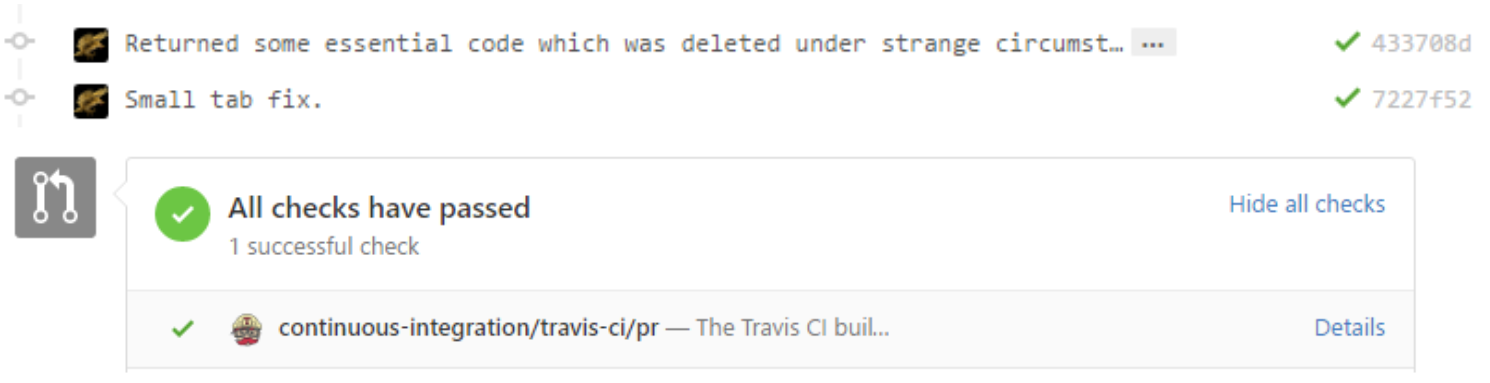
\includegraphics[width=0.7\textwidth]{travisSuccess.png}
\end{center}

Конфигурационный файл для случая, если у вас код на Java и проект прямо в корне репозитория, может выглядеть так:
\begin{minted}{yaml}
language: java
\end{minted}

Travis сам запустит maven или gradle, а они уже сделают что надо.

Сборку, естественно, можно настраивать как угодно. Есть понятие ``жизненный цикл сборки'', который описывает этапы, которые проходит собираемый проект, на каждом из этапов можно выполнять разные действия. Для Travis фазы жизненного цикла выглядят так:

\begin{itemize}
	\item Install apt addons --- на этом этапе устанавливаются пакеты из whitelist-а одобренных apt-пакетов. Такие пакеты можно ставить, даже если ваша конфигурация не разрешает sudo;
	\item before\_install --- действия перед установкой дополнительных зависимостей проекта;
	\item install --- установка дополнительных зависимостей (например, скачивание пакетов из maven-овских репозиториев для Java);
	\item before\_script --- перед началом исполнения скрипта собственно сборки;
	\item script --- скрипт сборки;
	\item after\_success или after\_failure --- команды, выполняемые после успешного завершения сборки или после проваленной сборки соответственно;
	\item \mintinline{text}|[OPTIONAL]| before\_deploy --- опциональный шаг перед выкладыванием результатов;
	\item \mintinline{text}|[OPTIONAL]| deploy --- опциональный шаг, выкладывание результатов куда-нибудь;
	\item \mintinline{text}|[OPTIONAL]| after\_deploy --- опциональный шаг, после завершения выкладывания результатов;
	\item after\_script --- команды, выполняемые после завершения сборки.
\end{itemize}

На самом деле, описание всех шагов в конфигурационном файле опционально, опциональные шаги отличаются тем, что они вообще не выполняются, если не указаны явно. И ещё Travis особо не ограничивает команды, выполняемые на фазах Install и Script, но если провалится команда на фазе Install, сборка получит статус ``errored'', а если на фазе Script, то ``failed''. Кстати, успешной считается сборка, где все выполняемые команды вернули код возврата 0, проваленной --- в противном случае. Так что скрипты сборки надо писать так, чтобы возвращать правильный код возврата.

Вот немного примеров конфигурационных файлов из реальных проектов:

\begin{itemize}
	\item Веб-приложение из нескольких сервисов на Java:
	\begin{itemize}
		\item \url{https://github.com/qreal/wmp/blob/master/.travis.yml}
	\end{itemize}
	\item Относительно большое десктопное приложение на C++:
	\begin{itemize}
		\item \url{https://github.com/qreal/qreal/blob/master/.travis.yml}
	\end{itemize}
	\item Билд в Docker-окружении (все зависимости носим с собой):
	\begin{itemize}
		\item \url{https://github.com/trikset/trikRuntime/blob/master/.travis.yml}
	\end{itemize}
\end{itemize}

И ещё один пример, как можно организовать сборку разных задач в домашке:

\begin{minted}{yaml}
language: java
os:
  - linux
env:
  - PROJECT_DIR=hw1
  - PROJECT_DIR=hw2
  - PROJECT_DIR=hw3
script: cd $PROJECT_DIR && ./gradlew check
\end{minted}

\section{AppVeyor}

Разумеется, Travis --- не единственная система непрерывной интеграции, в качестве примера ещё одной хочется рассказать про AppVeyor. Это тоже бесплатная для проектов с открытым исходным кодом CI-система, отличается от Travis тем, что качественно поддерживает Windows (и изначально создавалась как Windows-система, прежде всего для разработки приложений под .NET). Нам она интересна прежде всего тем, что она умеет и Java, а проверять ваши программы на собирабельность и работоспособность нелишне и под Linux, и под Windows. Тесты по-хорошему должны проходить и там, и там. AppVeyor использует для сборки Windows Server 2016 или Windows Server 2012 R2, Ubuntu 16.04.4 LTS или Ubuntu 18.04 LTS.

Конфигурируется сборка через appveyor.yml (либо .appveyor.yml), который тоже должен лежать в корне репозитория, кроме того, есть развитый web-GUI для конфигурирования сборки прямо с сайта AppVeyor-а. По умолчанию на фазе сборки в корне репозитория запускается система MSBuild, так что если вы пишете проект в Visual Studio и он у вас лежит прямо в корне репозитория, скорее всего, вообще ничего конфигурировать будет не надо. Для Java-проекта не уверен, что оно разберётся (хотя и не исключено), так что придётся всё-таки переопределить фазу сборки. У AppVeyor фазы жизненного цикла и синтаксис очень похожи на Travis, есть подробное описание (в отлиие от Travis, кстати): \url{https://www.appveyor.com/docs/appveyor-yml/}.

Пример реальной конфигурации достаточно большого проекта: \url{https://github.com/qreal/qreal/blob/master/appveyor.yml}.

Обратите внимание, что собирать двумя CI-серверами один проект не зазорно, и, хоть и не будет требоваться в домашке, это рекомендуется делать. Например потому, что работающая только на одной из ОС функциональность может привести к некоторому снижению баллов.

\section{CodeCov}

Помимо CI, при разработке используется ещё куча облачных инструментов. Следующая штука, которую хочется показать --- это средство для анализа тестового покрытия CodeCov (\url{https://codecov.io/}). На самом деле, эта штука сама тестовое покрытие считать не умеет, и даже тесты не исполняет, она просто использует функциональность, которая и так есть в компиляторах или библиотеках по подсчёту строк кода, исполнявшихся во время тестового прогона. CodeCov просто красиво её визуализирует и показывает прямо на GitHub (комментирует пуллреквест информацией о том, как изменилось бы тестовое покрытие, если бы пуллреквест был принят). Например, для Java (Kotlin, Scala) используется библиотека JaCoCo, с которой собирается проект, для C++/gcc --- ключ ``-coverage'', встроенный в компилятор.

Как подключить CodeCov к сборке, написано хорошо и подробно в документации, но вот пример того, как это делается из Travis:

\begin{minted}{yaml}
language: java

after_success:
  - bash <(curl -s https://codecov.io/bash)
\end{minted}

Теперь если сборка заканчивается успешно (и прошли юнит-тесты), исполняется скрипт, который скачивается прямо по ходу с codecov.io, он и заливает результаты прогона на CodeCov. При этом подключить JaCoCo к проекту придётся таки вручную в build.gradle или pom.xml, но там написано, как это сделать.

Вот пример для Android-приложения: \url{https://github.com/codecov/example-android/blob/master/.travis.yml}

Вообще, CodeCov хорош для того, чтобы понимать, на что именно надо писать тесты и следить, чтобы тестовое покрытие не ухудшалось. Однако надо помнить, что даже 100\% тестовое покрытие не говорит, что в вашем коде нет ошибок. Зато практика показывает, что если метод не покрыт тестами, он, скорее всего, не работает.

\section{Codacy}

Ещё одна полезная штука --- полноценный облачный статический анализатор кода Codacy (\url{https://www.codacy.com/}). На самом деле, это один из многих подобного рода инструментов, но конкретно он один из самых старых и развитых. Codacy умеет искать сразу много типичных ошибок в коде: потенциальные баги, стайлгайд, мёртвый код, проблемы с производительностью и т.д. При этом поддерживается много языков, в том числе Java, Kotlin, C\#, C++, Python, Scala. Codacy очень настраиваема, ей можно сказать, на что ругаться, на что нет, включив/выключив более сотни разных проверок. Может быть очень полезной штукой, но требует некоторых усилий по автоматизации, поэтому не так популярна, как более простые штуки типа BetterCodeHub, которые ничего толком не умеют, но легко интегрируются.

\section{Инструменты планирования}

Теперь немного про инструменты, которые сами с кодом ничего не делают, а помогают с сопутствующими задачами --- управлением проектом и коммуникациями. Первый инструмент, о котором вы, наверное, и сами слышали --- это Trello (\url{https://trello.com/}). Это легковесный инструмент планирования, реализованный как веб-приложение, бесплатный в базовом варианте и используемый не только в IT-сфере, но и везде, где надо что-то организовать, спланировать и упорядочить (вплоть до списка покупок в магазине).

Концептуально Trello представляет собой набор \textit{досок}, каждая доска состоит из \textit{списков}, каждый список состоит из \textit{карточек}. Карточни можно перетаскивать из списка в список, комментировать, снабжать тэгами, делать там списки (в том числе, TODO-списки, откуда можно вычёркивать сделанное), назначать им ответственных, дедлайны, прикладывать картинки и т.д. Типичная организация списков для IT-проектов --- это классические TODO, Doing, Done плюс возможные варианты типа Testing, Designing и т.д. Карточка соответствует одной короткой задаче и перетаскивается между списками. Например, член команды хочет взять себе задачу --- он записывает себя в карточку ответственным и перетаскивает её в Doing, остальные члены команды видят, что задача взята.

Trello не стоит использовать для стратегического планирования, потому что если карточек пара десятков, то ещё ладно, а если у вас взрослый проект с более сотни запросов от пользователей, багов и фич, которые надо сделать, то Trello использовать тяжеловато, потому как в карточках будет сложно ориентироваться. Тем не менее, Trello хорош для тактического планирования и отслеживания задач --- например, задач одной итерации большого проекта. Если проект маленький, то Trello идеален.

Более тяжеловесный инструмент планирования --- Pivotal Tracker (\url{https://www.pivotaltracker.com}). Он создавался уже конкретно для разработки ПО, даже более специфично --- для разработки ПО по методологии Scrum. Вообще, Scrum --- это самая популярная нынче из Agile-методологий, по которой разрабатываются практически все проекты сейчас (точнее, как правило, говорят, что разрабатываются, но на самом деле часто от методологи отступают). Методологические подробности будут в курсе ``Разработка ПО'', а нам сейчас важно, что проект разрабатывается короткими (от недели до месяца) итерациями, команда поддерживает список задач --- так называемый \textit{бэклог}, специально выделенный человек в команде приоритизирует задачи, двигая их вверх-вниз по бэклогу, вся команда оценивает задачи в условных единицах. Есть понятие ``скорость команды'' --- сколько условных единиц команда успевает сделать за одну итерацию. На текущую итерацию отбираются задачи из самого верха бэклога так, чтобы их суммарная оценка соответствовала скорости команды, они фиксируются на итерацию и команда начинает их делать. В Scrum нет тимлида, каждый член команды может сам взять себе задачу и начать её делать. В конце итерации проводится \textit{демо} с презентацией текущих результатов заказчику, либо очередной релиз.

Pivotal Tracker всё это поддерживает. Внешне всё выглядит как в Trello --- есть проект, в нём списки с задачами. Но списка всего три --- Icebox (что было бы неплохо сделать вообще, рано или поздно), Backlog (это уже оцененные и запланированные задачи) и Current (это задачи на текущую итерацию). Задачи можно оценивать в условных единицах, по шкале либо от 0 до 3, либо по фибоначчиевой шкале (0, 1, 2, 3, 5, 8), выбирается в настройках проекта. Задачи имеют тип --- feature, bug, chore (это разные рефакторинги и прочая деятельность по поддержанию кода, которая непосредственной пользы заказчику не приносит), и статус --- Unstarted, Started, Finished, Delivered, Accepted/Rejected, задачи двигаются по фиксированному жизненному циклу от Unstarted к Accepted. При этом автоматически считается скорость команды --- Pivotal Tracker ведёт статистику, сколько условных единиц функциональности было закрыто за итерацию, так что за несколько итераций получается довольно точная оценка реальной скорости команды. При этом на скорость влияют только задачи типа feature --- что реально полезного для заказчика команда успевает сделать за итерацию. Так что если команда целыми днями рефакторит код, чтобы довести его до совершенства, или исправляет свои баги, то скорость её будет низка и планировать много фич на итерацию Pivotal Tracker не позволит (конечно, его можно переубедить, скорость можно прописать вручную, да и задачи назначить на итерацию вручную, но он по крайней мере покажет, что вас может ждать провал). По моему личному опыту, через полгода аккуратного пользования Pivotal Tracker-ом он может предсказывать сроки выполнения этапов проекта с чудовищной точностью --- до плюс-минус пары дней при планировании на полгода. Разные отпуска/болезни/праздники, неточности оценок задач и разные тормозящие факторы усредняются (довольно быстро, на самом деле), и если в команде не происходит больших перемен, даже грубые оценки в среднем дают очень точный результат.

Есть поддержка релизов --- задачу можно пометить как релиз и назначить ему дедлайн, тогда Pivotal Tracker будет предупреждать, если считает, что с существующими запланированными до него задачами релиз не уложится к дедлайну. Есть тэги, по которым можно группировать и искать задачи. Есть epic-и --- это большие задачи, разделяемые на несколько подзадач, и прогресс по epic-у отслеживается по прогрессу по задачам, которые в него входят.

Pivotal Tracker ещё умеет некоторую аналитику --- например, рисовать \textit{burndown chart}-ы. Это график того, как закрываются задачи во время итерации --- по горизонтальной шкале откладывается время, по вертикальной --- количество условных единиц, которые ещё осталось сделать. Можно следить за поведением кривой ``сжигаемых'' в ходе разработки условных единиц, в начале итерации она должна быть где-то высоко, но в конце достичь нуля. Если кривая выше, чем надо, можно бить тревогу.

\section{Средства коммуникации}

Средства коммуникации проектной команды тоже на удивление важны в процессе разработки. Тут на самом деле обычно используется что угодно --- чаще всего почта, Skype, разные корпоративные мессенджеры (Microsoft Lync, который уже помер, Mattermost, который вполне жив). Некоторые пользуются и мессенджерами общего назначения, мы в былые времена пользовались Jabber-ом, затем перешли на Telegram. Такие мессенджеры не очень удобны в том плане, что лучше не смешивать деловое и личное общение, к тому же специализированные штуки имеют полезную функциональность типа возможности расшарить рабочий стол (хотя тут TeamViewer доминирует), подсветки кода, интеграции с багтрекером и системой контроля версий --- всё это обычные бытовые мессенджеры, как правило, не умеют.

Тут хотелось бы упомянуть средства, популярные в open source-мире --- Slack и Gitter. Они довольно легко интегрируются с CI и системами контроля версий, умеют синтаксическую подсветку кода, вложения, отображение картинок и т.д. Gitter в каком-то смысле более открыт --- по умолчанию не требует авторизации, чтобы читать сообщения, поэтому его часто используют для общения с сообществом, когда заинтересованных людей может быть много. Slack имеет понятие ``команда'' и по умолчанию никого извне не пускает, поэтому он популярен для более закрытых проектов, тем не менее, в open source его тоже используют. У Slack несколько получше с интеграцией с разными инструментами, но несколько похуже со скоростью работы (особенно десктопного клиента).

\section{Встроенные средства GitHub}

На самом деле, GitHub, которым вы и так пользуетесь, сам умеет очень многое. Во-первых, GitHub Issues --- встроенный багтрекер, можно включить в настройках для любого репозитория. По сравнению с более взрослыми багтрекерами его возможности довольно ограничены (нет жизненного цикла бага, кучи полей, которыми обычно пользуются, вложенных задач и т.д.), но много чего он всё-таки умеет: майлстоуны с возможностью привязывать к ним задачи и определять дедлайны, метки на багах (с помощью которых на самом деле симулируются и жизненный цикл бага, и всякие пол типа priority, которые багтрекерами обычно поддерживаются ``из коробки''),  возможность закрывать баги автоматически (если в сообщении коммита есть ``close'' или ``fix'' и \#<номер бага>). Для типичного open source-проекта багтрекер GitHub-а вполне ок, а то, что его не надо настраивать и он достаточно прост, чтобы люди со стороны могли писать вам баги --- дополнительные очки в его пользу (кстати, для обеспечения последнего можно определить шаблоны багов в markdown, тогда при создании нового бага будет сразу создаваться баг по шаблону). Обращаю внимание, что пуллреквест тоже считается Issue, попадает в GitHub Issues и ведёт себя как обычный баг --- его можно открывать/закрывать, назначать ответственного, ставить тэги и т.д., и даже ссылаться в коммитах и других issue через символ \#.

GitHub Projects --- инструмент планирования, в плане функциональности нечто среднее между Trello и Pivotal Tracker. Там тоже есть списки и карточки, которые можно перекладывать между списками, но при этом карточки могут быть привязаны к багам из GitHub Issues. На один репозиторий может быть несколько проектов на GitHub Projects.

GitHub Wiki --- викистраницы, куда можно выкладывать полезную информацию о проекте. Включаются в настройках репозитория, редактируются с использованием Markdown (GitHub flavored, так что там тоже можно ссылаться на баги через решётку, делать красивую синтаксическую подсветку для разных языков и т.д.). Ещё, кстати, GitHub Wiki --- это тоже гитовый репозиторий, так что, во-первых, он ведёт историю ваших изменений, во-вторых, его можно склонит и редактировать локально.

GitHub Pages --- хостинг для статических сайтов. Хостит HTML с JavaScript, которы берёт либо из ветки gh-pages проекта, либо из отдельного репозитория, смотря как настроите. Сайту выделяется доменное имя ``<имя проекта>.github.io'' (бесплатно). Многие проекты таким образом хостят свою документацию, как пользовательскую, так и техническую. 

+2 балла к домашке за настроенный CI так, чтобы он собирал JavaDoc и деплоил его на GitHub Pages, и при этом у вас не украли бы пароль от репозитория.

\section{Авторское право}

Последний, но немаловажный аспект, касающийся open source --- это авторское право. На самом деле это вообще часто забываемый, но весьма важный при разработке ПО вопрос. Дело в том, что даже если код лежит на GitHub и типа в свободном доступе, его далеко не всегда можно переиспользовать в своих проектах. Вообще, международное (и, соответственно, российское) законодательство устроено так, что плодами интеллектуальной деятельности легально можно пользоваться только в том случае, если автор это явно разрешил. Поэтому если вы скопипастили кусок кода с чьего-то репозитория без лицензии в свой проект, актор может вас засудить за кражу интеллектуальной собственности. Так что просто код на GitHub --- это не совсем open source.

Немного подробнее про результаты интеллектуальной деятельности и авторское право. Бывают исключительные и личные неимущественные права. Личные неимущественные права --- это право называться автором произведения, право заявлять, что вы автор и т.д., личные неимущественные права неотчуждаемы --- то есть их нельзя передать и нельзя забрать. Если ваш работодатель пишет в трудовом договоре, что вы не имеете права говорить, что вы писали этот код, этот пункт трудового договора может быть признан недействительным, поскольку противоречит законодательству. Личные неимущественные права называются неимущественными, поскольку всё равно никакого дохода автору не приносят.

Исключительные права можно передать. Исключительные права --- например, право пользоваться произведением, право воспроизводить, модифицировать, продавать и т.д. и т.п. Мало кто знает, что и личные неимущественные права, и исключительные права начинают действовать в момент создания произведения, и принадлежат автору произведения, никакой регистрации или юридического оформления прав не требуется. Единственное, но очень важное исключение --- если произведение создано по служебному заданию, исключительные права на него принадлежат работодателю, так что написать плагин для IDEA в JetBrains и отсудить у JetBrains пару миллионов за то, что они им пользуются, не получится. Обычно это явно прописано в трудовом договоре, но даже если нет, то это всё равно есть в законе об авторском праве. Знаменитый знак копирайта \textcopyright служит только для информирования о правах и не требуется для их существования (то есть если у вас нигде не написано \textcopyright, это никак не влияет на ваши права на произведение). Да, просто кусок кода --- это тоже произведение и тоже охраняется законом об авторском праве.

Некоторая тонкость в том, что соавторы владеют произведением в равной степени, если произведение невозможно явно разделить между ними. Так что если кто-то закоммитит в ваш проект пару строк кода, он становится таким же автором, как и вы, со всеми вытекающими последствиями --- вам надо будет спрашивать согласие соавтора на передачу исключительных прав (в том числе, продажу или смену лицензии).

И ещё одна тонкость --- идея не охраняется, охраняется её физическое выражение. Люди, бегающие и кричащие, что у них есть замечательная идея для стартапа, с точки зрения законодательства на самом деле не имеют ничего. И неспроста --- от идеи до реализации большой путь, и если у вас только идея, то это ещё ничего не значит. Зато если вашу замечательную идею украдут и сделают стартап раньше вас, то законы вас не защитят.

Лицензия --- это на самом деле юридически правильный способ передать часть прав на поизведение. Если вы хотите, чтобы вашим кодом всё-таки пользовались, лицензия вам необходима, благо GitHub предлагает выложить лицензию из набора популярных при создании репозитория, да ещё и объясняет, какая вам больше подойдёт. Пример лицензии ---``Do what the **** you want to public license'' (WT*PL\footnote{https://en.wikipedia.org/wiki/WTFPL}), которая звучит примерно так:
\begin{minted}{text}
DO WHAT THE **** YOU WANT TO PUBLIC LICENSE
                   Version 2, December 2004
 
Copyright (C) 2004 Sam Hocevar <sam@hocevar.net>

Everyone is permitted to copy and distribute verbatim or modified
copies of this license document, and changing it is allowed as long
as the name is changed.
 
           DO WHAT THE **** YOU WANT TO PUBLIC LICENSE
  TERMS AND CONDITIONS FOR COPYING, DISTRIBUTION AND MODIFICATION

 0. You just DO WHAT THE **** YOU WANT TO.
 \end{minted}

К несчастью, ``Want to'' может включать в себя патентование произведения и подачу в суд на автора за нарушение патента (и такие дела реально практикуются патентными троллями), поэтому обычно лицензии более длинны и унылы, даже если хотя сказать примерно то же самое. Кстати,в России и Европе программы не патентуют, в США --- да. В России зато можно получить свидетельство о регистрации программы для ЭВМ, это не очень сложная бюрократическая процедура, которая ничего не даёт, кроме плюс пары баллов при поступлении в магистратуру СПбГУ и возможности формально доказать своё авторство, если вы стали жертвой тролля, пытающегося похитить вашу интеллектуальную собственность.

Общее правило таково, что каждый нормальный open source-проект должен иметь лицензию. Так что начиная с сегодняшнего дня в домашке лицензия обязательна.

Часто используемые open source-лицензии:

\begin{itemize}
	\item GPL, LGPL. GPL вирусная, поэтому использовать её, внезапно, плохая практика. Она создавалась, чтобы подбодрить развитие свободного ПО, поэтому содержит фразу, что ПО, использующее ПО под GPL, само должно быть лицензировано под GPL. В светлом мире GPL-апологетов в конечном итоге всё будет лицензировано под GPL, так что эта фраза не будет иметь значение. В суровой реальности же это очень мешает, потому что серьёзные компании не используют GPL как лицензию, следовательно, весь код, лицензированный под GPL, для них просто не существует. Есть LGPL (Library- или Light-), разрешающая линковаться к GPL-коду, не ``заражаясь'' GPL-лицензией, но включать GPL- код как код всё так же не позволяющая (беда C++никам с их заголовочными файлами). Кстати, есть распространённое заблуждение, что код под GPL должен распространяться бесплатно --- это неправда, лицензия требует лишь, чтобы тот, кому вы продали бинарные файлы, мог получить и код, и имел бы право его модифицировать (при условии, что модификации тоже будут под GPL). Есть ещё Affero GPL, которая касается веб-приложений и требует, чтобы если приложением можно пользоваться по сети, должно быть можно получить его код (GPL такого требовать не могла, потому что у веб-приложений формально бинарники никому не передаются).
	\item MIT License --- разрешающая лицензия, не обладает вирусностью GPL, разрешает пользоваться кодом в том числе и в проектах с другими лицензиями (вклчая коммерческие). Запрещает лишь ``воровать'' интеллектуальную собственность, например, объявив себя единственным обладателем прав на продажу проекта.
	\item Apache License 2.0 устроена примерно как MIT License, но может применяться пофайлово, а не ко всему проекту целиком, и имеет ряд тонкостей, касающихся патентов. Apache License считается более длинной и тяжёлой в применении (она обычно подразумевает наличие шапки с краткой формой лицензии в каждом файле), но более юридически аккуратной, поэтому всенародно любима.
	\item BSD License (в разных вариантах) --- тоже разрешающая лицензия, короткая и по делу.
	\item The Unlicense --- явная передача произведения в Public Domain. Public Domain (или общественное достояние, если по-русски) --- это юридический термин, означающий произведения, имущественные права на которые не существуют --- либо истекли по давности (у нас это 75 лет, кажется), либо автор от них явно отказался. Отказаться от имущественных прав грамотно --- хорошо и правильно, поскольку ими тогда никто не может завладеть и патентные тролил останутся ни с чем, а вашим произведением все смогут пользоваться (что, в конечном итоге, цель всего open source и вообще любого достойного человека).
	\item Семейство лицензий Creative Commons --- лицензии прежде всего не для софта, а для разных ресурсов (картинок, текстов и т.д.).
\end{itemize}

\end{document}
